%index
\chapter{INTRODUCCI�N}
\section{LO ESCRITO SOBRE EL TEMA}
\section{MARCO TE�RICO}
\subsection{C\'AMARA CON SENSOR DE PROFUNDIDAD}
Seg�n el estudio, On the performance of the Intel SR300 depth camera: metrological and critical characterization \cite{carfagni2017performance}, menciona que unas de las principales funciones de las \acrfull{RGBD} es adquirir y procesar datos en \acrfull{TRESD}, estas c�maras se han utilizado en el sector industrial y acad�mico en aplicaciones tales como: La localizaci�n y mapeo simult�neos, reconocimiento de posiciones y gestos e ingenier�a inversa. \\
Por otro lado el estudio, RGB-D mapping: Using Kinect-style depth cameras for dense 3D modeling of indoor environments   \cite{carfagni2017performance}, indica que las c�maras con sensor de profundidad capturan p�xeles de informaci�n de im�genes (RGB) y de profundidad, tal como se muestra en la siguiente figura:
\begin{figure}[h]
	\caption{Captura de datos de una c�mara con sensor de profundidad}
	\label{fig:RGBD}
	\centering
	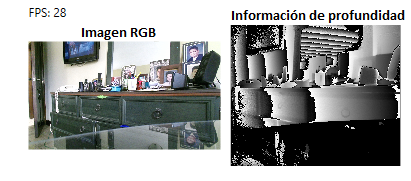
\includegraphics[]{graphics/RGB-D.PNG} \\
	\textbf{Fuente:} Tomado por el autor de tesis
\end{figure}  \\
La figura \ref{fig:RGBD}, fue capturado por el dispositivo, Kinect de XBox One, a una velocidad de 28 \acrfull{FPS}, cabe mencionar que los p�xeles  blancos de la imagen de la derecha, no se puede determinar el valor de profundidad, debido que falta el an�lisis de distancia, angulo relativo de la superficie, material de superficie, y otras variable m�s que se observar� en el presente trabajo.
\section{TRABAJOS RELACIONADOS}